%package list
\documentclass{article}
\usepackage[top=3cm, bottom=3cm, outer=3cm, inner=3cm]{geometry}
\usepackage{multicol}
\usepackage{graphicx}
\usepackage{url}
\usepackage{hyperref}
\usepackage{array}
\newcolumntype{x}[1]{>{\centering\arraybackslash\hspace{0pt}}p{#1}}
\usepackage{natbib}
\usepackage{pdfpages}
\usepackage{multirow}
\usepackage[normalem]{ulem}
\useunder{\uline}{\ul}{}
\usepackage{svg}
\usepackage{xcolor}
\usepackage{listings}
\lstdefinestyle{ascii-tree}{
    literate={├}{|}1 {─}{--}1 {└}{+}1 
  }
\lstset{basicstyle=\ttfamily,
  showstringspaces=false,
  commentstyle=\color{red},
  keywordstyle=\color{blue}
}
%\usepackage{booktabs}
\usepackage{caption}
\usepackage{subcaption}
\usepackage{float}
\usepackage{array}

% Comment
\usepackage{verbatim}

\newcolumntype{M}[1]{>{\centering\arraybackslash}m{#1}}
\newcolumntype{N}{@{}m{0pt}@{}}


%%%%%%%%%%%%%%%%%%%%%%%%%%%%%%%%%%%%%%%%%%%%%%%%%%%%%%%%%%%%%%%%%%%%%%%%%%%%
%%%%%%%%%%%%%%%%%%%%%%%%%%%%%%%%%%%%%%%%%%%%%%%%%%%%%%%%%%%%%%%%%%%%%%%%%%%%
\newcommand{\itemEmail}{rzapata@unsa.edu.pe}
\newcommand{\itemStudent}{Reyser Julio Zapata Butrón}
\newcommand{\itemCourse}{Análisis Y Diseño de Algoritmos}
\newcommand{\itemCourseCode}{1702231}
\newcommand{\itemSemester}{IV}
\newcommand{\itemUniversity}{Universidad Nacional de San Agustín de Arequipa}
\newcommand{\itemFaculty}{Facultad de Ingeniería de Producción y Servicios}
\newcommand{\itemDepartment}{Departamento Académico de Ingeniería de Sistemas e Informática}
\newcommand{\itemSchool}{Escuela Profesional de Ingeniería de Sistemas}
\newcommand{\itemAcademic}{2024 - B}
\newcommand{\itemInput}{24 septiembre 2024}
\newcommand{\itemOutput}{24 septiembre 2024}
\newcommand{\itemPracticeNumber}{02}
\newcommand{\itemTheme}{Búsqueda en vector ordenado. Búsqueda Binaria}
\newcommand{\itemPracticeDuration}{02 horas}
%%%%%%%%%%%%%%%%%%%%%%%%%%%%%%%%%%%%%%%%%%%%%%%%%%%%%%%%%%%%%%%%%%%%%%%%%%%%
%%%%%%%%%%%%%%%%%%%%%%%%%%%%%%%%%%%%%%%%%%%%%%%%%%%%%%%%%%%%%%%%%%%%%%%%%%%%

\usepackage[english,spanish]{babel}
\usepackage[utf8]{inputenc}
\AtBeginDocument{\selectlanguage{spanish}}
\renewcommand{\figurename}{Figura}
\renewcommand{\refname}{Referencias}
\renewcommand{\tablename}{Tabla} %esto no funciona cuando se usa babel
\AtBeginDocument{%
	\renewcommand\tablename{Tabla}
}

\usepackage{fancyhdr}
\pagestyle{fancy}
\fancyhf{}
\setlength{\headheight}{30pt}
\renewcommand{\headrulewidth}{1pt}
\renewcommand{\footrulewidth}{1pt}
\fancyhead[L]{\raisebox{-0.2\height}{
\includegraphics[width=3cm]{img/logo_episunsa.png}}}
\fancyhead[C]{\fontsize{7}{7}\selectfont	\itemUniversity \\ \itemFaculty \\ \itemDepartment \\ \itemSchool \\ \textbf{\itemCourse}}
\fancyhead[R]{\raisebox{-0.2\height}{
\includegraphics[width=1.2cm]{img/logo_abet}}}
\fancyfoot[L]{Reyser Julio Zapata Butrón}
\fancyfoot[C]{\itemCourse}
\fancyfoot[R]{Página \thepage}

% Estilos del Código
\usepackage{listings}
\usepackage{color, colortbl}
\definecolor{dkgreen}{rgb}{0,0.6,0}
\definecolor{gray}{rgb}{0.5,0.5,0.5}
\definecolor{codebackground}{rgb}{89, 0.97, 0.90}
\definecolor{tablebackground}{rgb}{0.8, 0, 0}

\lstset{
  language=C++,                  
  basicstyle=\ttfamily\footnotesize,
  keywordstyle=\color{blue},     
  commentstyle=\color{dkgreen},    
  stringstyle=\color{red},       
  backgroundcolor= \color{codebackground},
  numbers=left,                  
  numberstyle=\tiny\color{gray},
  stepnumber=1,                  
  numbersep=5pt,                
  showspaces=false,              
  showstringspaces=false,      
  showtabs=false,                
  frame=single,                  
  captionpos=b,                  %
}

\begin{document}
	\vspace*{10px}
	
	\begin{center}	
		\fontsize{17}{17} \textbf{ Informe de Laboratorio \itemPracticeNumber}
	\end{center}

 %% TABLA %%
 
	\centerline{\textbf{\Large Tema: \itemTheme}}

	\begin{flushright}
		\begin{tabular}{|M{2.5cm}|N|}
			\hline 
			\rowcolor{tablebackground}
			\color{white} \textbf{Nota}  \\
			\hline 
			     \\[30pt]
			\hline 			
		\end{tabular}
	\end{flushright}	

	\begin{table}[H]
		\begin{tabular}{|x{4.7cm}|x{4.8cm}|x{4.8cm}|}
			\hline 
			\rowcolor{tablebackground}
			\color{white} \textbf{Estudiante} & \color{white}\textbf{Escuela}  & \color{white}\textbf{Asignatura}   \\
			\hline 
			{\itemStudent \par \itemEmail} & \itemSchool & {\itemCourse \par Semestre: \itemSemester \par Código: \itemCourseCode}     \\
			\hline 			
		\end{tabular}
	\end{table}		
	
	\begin{table}[H]
		\begin{tabular}{|x{4.7cm}|x{4.8cm}|x{4.8cm}|}
			\hline 
			\rowcolor{tablebackground}
			\color{white}\textbf{Laboratorio} & \color{white}\textbf{Tema}  & \color{white}\textbf{Duración}   \\
			\hline 
			\itemPracticeNumber & \itemTheme & \itemPracticeDuration   \\
			\hline 
		\end{tabular}
	\end{table}
	
	\begin{table}[H]
		\begin{tabular}{|x{4.7cm}|x{4.8cm}|x{4.8cm}|}
			\hline 
			\rowcolor{tablebackground}
			\color{white}\textbf{Semestre académico} & \color{white}\textbf{Fecha de inicio}  & \color{white}\textbf{Fecha de entrega}   \\
			\hline 
			\itemAcademic & \itemInput &  \itemOutput  \\
			\hline 
		\end{tabular}
	\end{table}

 %% CONTENIDO %%
\section{Código Fuente}
    El siguiente código es el que se usará para analizar los ejercicios propuestos en el laboratorio.
    \\
    \lstinputlisting[language=C++, caption={main.cpp}, numbers=left]{src/main.cpp}

    \textbf{Ejecución del código}
        \begin{figure}[H]
        	\centering
         	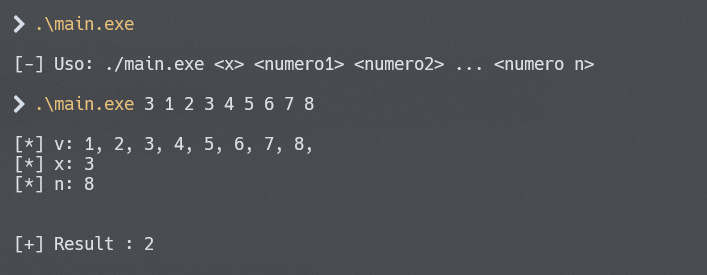
\includegraphics[width=0.8\textwidth,keepaspectratio]{img/main.png}
        \end{figure}

\section{Ejercicios}
    \subsection{Ejercicio 1}
        \begin{itemize}
            \item Para evitar valores de índice fuera del rango \(0..n-1\), podríamos cambiar la línea \(i = -1; d = n\) de la función \texttt{busquedaBinaria} a través de las siguientes tres líneas. Analice esta variante de código.

            \begin{verbatim}
            if (v[n-1] < x) return n;
            if (x <= v[0]) return 0;
            // ahora v[0] < x <= v[n-1]
            i = 0; d = n-1;
            \end{verbatim}
        \end{itemize}

        El cambio introduce dos condiciones adicionales antes de iniciar el ciclo \texttt{while}, lo cual garantiza que no se intenten acceder a índices fuera del rango permitido. La condición \texttt{if (v[n-1] < x)} maneja el caso en que el valor buscado \( x \) es mayor que todos los valores del vector, devolviendo \( n \) como el índice en el que debería estar \( x \) (justo después del último elemento). Por otro lado, \texttt{if (x <= v[0])} devuelve \( 0 \) si \( x \) es menor o igual al primer valor del vector, lo que indica que \( x \) debería estar al principio.\\\\
        En conclusión, las líneas de código añadidas nos aseguran que el valor buscado está dentro del rango ( (v[0], v[n-1] ), y por eso se ajustan los valores de \( i \) a \( 0 \) y \( d \) a \( n-1 \).

    \subsection{Ejercicio 2}
        \begin{itemize}
            \item Responda las siguientes preguntas sobre la función \texttt{busquedaBinaria}. ¿Qué sucede si \texttt{while (i < d-1)} se reemplaza por \texttt{while (i < d)}? O por \texttt{while (i <= d-1)}? ¿Qué pasa si intercambiamos \texttt{(i + d)/2} por \texttt{(i + d - 1)/2} o por \texttt{(i + d + 1)/2} o por \texttt{(d - i)/2}? ¿Qué sucede si \texttt{if (v[m] < x)} se reemplaza por \texttt{if (v[m] <= x)}? ¿Qué sucede si \texttt{i = m} se reemplaza por \texttt{i = m+1} o por \texttt{i = m-1}? ¿Qué sucede si \texttt{d = m} se reemplaza por \texttt{d = m+1} o \texttt{d = m-1}? 
        \end{itemize}

        \subsubsection*{a. Cambios en el ciclo \texttt{while (i < d-1)}}
            \begin{itemize}
                \item \textbf{Reemplazo por \texttt{while (i < d):}} Esto rompe el invariante, ya que el ciclo continuará hasta que \( i == d \), lo cual no pasará, ya que \( i \) nunca debería igualarse a \( d \) en el algoritmo. Esto lleva a una \textbf{condición infinita}.
                
                \item \textbf{Reemplazo por \texttt{while (i <= d-1):}} Al modificar esto, ocurre algo similar con la anterior modificación, generará una \textbf{condición infinita}.
            \end{itemize}
            
        \subsubsection*{b. Cambios en el cálculo de \texttt{(i + d)/2}}
            
            \begin{itemize}
                \item \textbf{Reemplazo por \((i + d - 1)/2:\)} Esto moverá el valor de \( m \) hacia la izquierda, haciendo que el algoritmo converja más rápido en algunos pocos casos, pero podría perder el valor correcto si no se ajustan las condiciones para actualizar \( i \) y \( d \) en base a esta nueva lógica.
                
                \item \textbf{Reemplazo por \((i + d + 1)/2:\)} Similar a la modificación anterior, pero esta vez moverá el valor de \( m \)  hacia la derecha, lo cual también afectará la convergencia y requeriría ajustes en la lógica de actualización de \( i \) y \( d \).
                
                \item \textbf{Reemplazo por \((d - i)/2:\)} Esto romperá la lógica del algoritmo, ya que cambia completamente el cálculo del punto medio.
            \end{itemize}
            
        \subsubsection*{c. Cambios en la condición \texttt{if (v[m] < x):}}
            
            \begin{itemize}
                \item \textbf{Reemplazo por \texttt{if (v[m] <= x):}} Esto altera el resultado del algortimo. En lugar de buscar el punto exacto donde \( x \) se encuentra entre \( v[i] \) o \( v[d] \), se permitiría que \( v[m] == x \) pase al siguiente lado de la búsqueda, lo cual lleva a resultados incorrectos al intentar encontrar el \textbf{índice correcto}.
            \end{itemize}
            
        \subsubsection*{d. Cambios en la asignación de \( i = m \):}
            
            \begin{itemize}
                \item \textbf{Reemplazo por \( i = m+1:\)} Esto altera el algoritmo, ya que al poner \( m+1 \) afecta el valor de retorno, en muchos casos sumandole al resultado, generando un \textbf{indice incorrecto}.
                
                \item \textbf{Reemplazo por \( i = m-1:\)} Esto rompe el algoritmo, ya que estamos retrocediendo innecesariamente, lo cual genera en un \textbf{ciclo infinito}.
            \end{itemize}
            
        \subsubsection*{e. Cambios en la asignación de \( d = m \):}
            \begin{itemize}
                \item \textbf{Reemplazo por \( d = m+1:\)} Esto rompe el algortimo, al mover \textbf{d} a la derecha con \( m+1 \) genera una \textbf{condición infinita}.
                
                \item \textbf{Reemplazo por \( d = m-1:\)} Esto rompe el algoritmo, al mover \textbf{d} a la izquierda con \( m-1 \) en muchos casos genera un \textbf{retorno incorrecto} o una \textbf{condicion infninita}.
            \end{itemize}

    \subsection{Ejercicio 3}
        \begin{itemize}
            \item Ejecute la función \texttt{busquedaBinaria} con \(n = 16\). ¿Cuáles son los valores posibles de \(m\) en la primera iteración? ¿Cuáles son los posibles valores de \(m\) en la segunda iteración? ¿En la tercera? ¿En la cuarta?
        \end{itemize}

        \textbf{1. Primera iteración:} Siempre será 7.

        \textbf{2. Segunda iteración:} Los posibles valores son 3 y 11.

        \textbf{3. Tercera iteración:} Los posibles valores son 1, 5, 9, 13.

        \textbf{4. Cuarta iteración:} Los posibles valores son 0, 2, 4, 6, 8, 10, 12, 14.

        \textbf{5. Quinta iteración:} El único valor posible es 15.

    \subsection{Ejercicio 4}
        \begin{itemize}
            \item En la función \texttt{busquedaBinaria}, ¿es cierto que \(m\) está en \(0..n-1\) siempre que se ejecuta la sentencia \texttt{if (v[m] < x)}? (Tenga en cuenta que \(i\) y \(d\) pueden no estar en \(0..n-1\).)
        \end{itemize}

        Sí, porque en cada iteración \( m \) se calcula como \( \frac{i + d}{2} \), y tanto \( i \) como \( d \) siempre están en el rango de \([-1, n]\). Como el ciclo while se detiene antes de que \( i == d \), \( m \) siempre se encuentra dentro de los límites de \( 0..n-1 \).

    \subsection{Ejercicio 5}
        \begin{itemize}
            \item Variantes de algoritmos. Escriba una versión de la función de \texttt{busquedaBinaria} que tenga la siguiente invariante: al comienzo de cada iteración, \(v[i-1] < x \leq v[d]\). Repita con \(v[i-1] < x \leq v[d+1]\). Repita con \(v[i] < x \leq v[d+1]\).
        \end{itemize}

        \textbf{Con invariante \( v[i-1] < x \leq v[d] \):}
            \begin{verbatim}
            int busquedaBinaria(int x, int n, int v[]) {
                int i = 0, d = n;
                while (i < d) {
                    int m = (i + d) / 2;
                    if (v[m] < x) i = m + 1;
                    else d = m;
                }
                return d;
            }
            \end{verbatim}
        
        \textbf{Con invariante \( v[i-1] < x \leq v[d+1] \):}
            \begin{verbatim}
            int busquedaBinaria(int x, int n, int v[]) {
                int i = 0, d = n - 1;
                while (i <= d) {
                    int m = (i + d) / 2;
                    if (v[m] < x) i = m + 1;
                    else d = m - 1;
                }
                return i;
            }
            \end{verbatim}
        
        \textbf{Con invariante \( v[i] < x \leq v[d+1] \):}
            \begin{verbatim}
            int busquedaBinaria(int x, int n, int v[]) {
                int i = 0, d = n - 1;
                while (i <= d) {
                    int m = (i + d) / 2;
                    if (v[m] <= x) i = m + 1;
                    else d = m - 1;
                }
                return i;
            }
            \end{verbatim}  


%%% REPOSITORIO DE GITHUB %%%

\section{Repositorio de Github}
	\begin{itemize}
		\item Repositorio de Github donde se encuentra el actual laboratorio \\
		\url{https://github.com/ReyserLynnn/ada-lab-b-24b/tree/main/laboratorio02/src}

        \item Repositorio de Github donde se encuentran los laboratorios del curso\\
		\url{https://github.com/ReyserLynnn/ada-lab-b-24b.git}
	\end{itemize}

\begin{comment}
\section{Referencias}
\begin{itemize}			
	\item \url{https://dialnet.unirioja.es/servlet/articulo?codigo=4573315}
\end{itemize}	    
\end{comment}

\end{document}